\let\negmedspace\undefined
\let\negthickspace\undefined
\documentclass[journal,12pt,twocolumn]{IEEEtran}
\usepackage{cite}
\usepackage{amsmath,amssymb,amsfonts,amsthm}
\usepackage{algorithmic}
\usepackage{graphicx}
\usepackage{textcomp}
\usepackage{xcolor}
\usepackage{txfonts}
\usepackage{listings}
\usepackage{enumitem}
\usepackage{mathtools}
\usepackage{gensymb}
\usepackage{comment}
\usepackage[breaklinks=true]{hyperref}
\usepackage{tkz-euclide} 
\usepackage{listings}
\usepackage{gvv}                                        
\def\inputGnumericTable{}                                 
\usepackage[latin1]{inputenc}                                
\usepackage{color}                                            
\usepackage{array}                                            
\usepackage{longtable}                                       
\usepackage{calc}                                             
\usepackage{multirow}                                         
\usepackage{hhline}                                           
\usepackage{ifthen}                                           
\usepackage{lscape}
\usepackage{caption}
\newtheorem{theorem}{Theorem}[section]
\newtheorem{problem}{Problem}
\newtheorem{proposition}{Proposition}[section]
\newtheorem{lemma}{Lemma}[section]
\newtheorem{corollary}[theorem]{Corollary}
\newtheorem{example}{Example}[section]
\newtheorem{definition}[problem]{Definition}
\newcommand{\BEQA}{\begin{eqnarray}}
\newcommand{\EEQA}{\end{eqnarray}}
\newcommand{\define}{\stackrel{\triangle}{=}}
\theoremstyle{remark}
\newtheorem{rem}{Remark}
\begin{document}

\bibliographystyle{IEEEtran}
\vspace{3cm}

\title{10.5.2.14}
\author{EE23BTECH11003 - pranav}
\maketitle
\newpage

\bigskip
\renewcommand{\thefigure}{\arabic{figure}}
\renewcommand{\thetable}{\arabic{table}}

\textbf{Question}:
How many multiples of 4 lie between 10 and 250?\\
\solution
\begin{table}[h]
    \centering
    \input{tables/Table.Tex}
    \caption{Variables Used}
    \label{tab:table_11.9.3.6}
\end{table}
\begin{align}
     4n_{1}>10   \text{ and }  4n_{2}<250  \\
\implies n_{1}=3,n_{2}=62  \quad (\text{as }  n \in \mathbb{N})
\end{align}
 $\therefore$ number of multiples of 4 which lie between  10 and 250 are $62-3+1=60$ \\
considering the series to start from $n=0$ the general term
\begin{align}
X(n)&=[X(0)+n\cdot d].u(n)\\
X(n)&=4n.u(n)
\end{align}
\begin{figure}[h!]
    \centering
    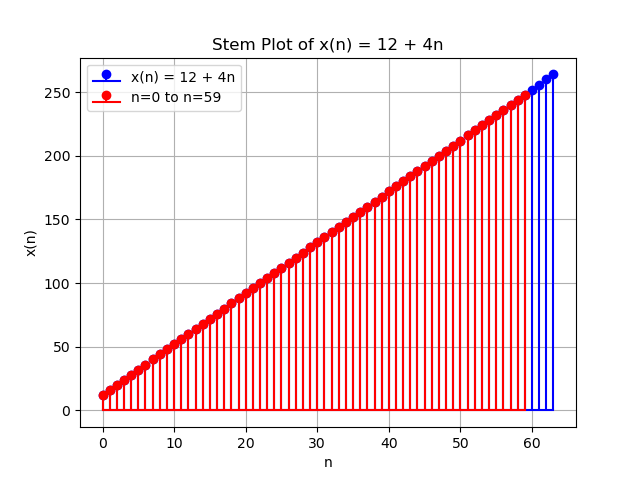
\includegraphics[width=1.1\linewidth]{figs/graph1.png}
    \caption{stem plot of $X(n)$}
\end{figure}

applying Z transform
\begin{align}
    X(z)&= \sum_{n=-\infty}^{\infty}X(n)\cdot z^{-n}\\
   \implies X(z)&= \sum_{n=-\infty}^{\infty} 4n\cdot u(n)\cdot z^{-n}\\
   \implies X(z) &=\sum_{n= 0}^{\infty} 4n \cdot z^{-n}\\
   \text{from } \ref{eq:11.9.5.26.2}\\
   \implies X(z)&=\frac{4\cdot z^{-1}}{(1-z^{-1})^{2}}
\end{align}
\end{document}
